Going back to the Bayesian framework, so far, we collected data about a phenomenon, used this data to update our prior belief into the posterior belief \cref{eq:bayes_rule}, then use the posterior to form our predictive distribution for new inputs \cref{eq:bayesian_predictive}.
Recall the posterior predictive
$$
    \pdf{y|x; \mathcal{D}}=  \int \pdf{\theta | \mathcal{D}}\, \pdf{y|\theta, x} \, d\theta
$$


The epistemic uncertainty comes from compounding two factors, the uncertainty in $\pdf{\theta | \mathcal{D}}$, and the \emph{disagreement} between the parameters with high posterior probability  $\pdf{\theta | \mathcal{D}}$. 
To unpack this, the uncertainty in $\pdf{\theta | \mathcal{D}}$ is simply how spread out the posterior is over different parameter settings. For instance, if the posterior is Gaussian, then the higher the variance of that Gaussian the higher the uncertainty is. Intuitively, this is saying we have not seen enough data to be sure what the correct parameters are.

However, the uncertainty over parameters does not directly translate into uncertainty in the posterior predictive distribution. This also depends on how much the predictions from those different parameters diverge. Being uncertain over a wide range of parameters which all give the same prediction, will result in no epistemic uncertainty in the predictive distribution. On the other hand, having a posterior concentrated over a few parameter settings which have large differences in their predictions can result in high epistemic uncertainty. In an ideal setting, the posterior predictive distribution captures all our epistemic uncertainty; \cref{eq:bayesian_predictive} gives the \emph{correct} predictive distribution. However, we will see in the next section that there are realistic settings where the an assumption of Bayes rule is broken, and how this might results in \emph{incorrect} predictive distributions. 


\subsection{Epistemic uncertainty under distribution shift}
\label{sec:epistemic_shift}

The Bayesian framework, alongside most other practical ML approaches~\citep[chapter~5]{goodfellow2016deep}, assume the training data is independently and identically distributed(i.i.d) from the target distribution, the target distribution being the one we intend to perform inference on. Problems arise when this assumption is broken.
Let the target distribution be $\pdf{x,y} = \pdf[target]{x} \pdf{y|x}$.
We consider a scenario where the training data is drawn i.i.d from a training distribution which is different form the target distribution, $\pdf{x,y} = \pdf[train]{x} \pdf{y|x}$. Thus the problem is that the distribution over the inputs is different from training to inference. 
Intuitively the image we have is that \pdf[target]{x} is a \emph{wider} distribution capturing all possible inputs, and \pdf[train]{x} concentrates its probability on a sub-region of \pdf[target]{x}. We refer to inputs which occur frequently in \pdf[target]{x} but not in \pdf[target]{x} as Out-Of-Distribution~(OOD).

The problem is that the model could be asked at inference time to make predictions over input regions where it has seen no data. \Cref{fig:uncertainty_toy} shows three possible posterior predictive distribution, all identical in the region from zero to fifty. We also have some training samples in that region. All three distributions are equally consistent with the data, so which one of those should we get if we ran a Bayesian learning algorithm on the data?

It depends on the priors and other underlying assumptions. If we choose the \emph{right} prior for our problem we may end up with a distribution that closely matches the true distribution we are modelling. However, if we do not know the right prior, we cannot be confident that we got a reasonable answer. Note that we are not only risking getting incorrect mean predictions, but also incorrect uncertainty estimates. Therein lies the problem with the Bayesian approach when the i.i.d assumption is broken. There is a component of uncertainty which is not accounted for. Note that this is not the case when data is i.i.d, where with enough data, a poor choice of prior can be overcome. 


% \chmp{
    
%     I got confused by looking at the wrong figure first. However, I also believe that you can make your argument strong by
%     switching the discussion around. First start with a dataset and the two different sampling processes for the training data.
%     And then discuss the potential beliefs about the unseen points that are compatible with the observed data in case of the right 
%     example. (I.e., there is only one dataset, but different beliefs about unseen data).
    
%     Why are there different datasets? And why does the conditional distribution differ? If you assume $P(y|x)$ is the 
%     data generating process, there is no need to assume the generative process changes between intervals, but only that 
%     we have limited knowledge.
    
%     I would frame the whole discussion in the way of talking about a underlying data generating process, but different ways
%     to sample the training data. I.e., there is only one true curve, but in the right example we only see the linear part,
%     in the left example we see the samples from the whole domain.
    
%     I also have the impression that you are repeating yourself a couple of times. If you wanted to, you should be able to shorten
%     the section.
% }

% \Cref{fig:uncertainty_toy} shows samples from three datasets. The universal input distribution \dist{u} is the same for all three. 
% We split the input domain into two intervals, then we define \pdf{y|x} to be the same for all three datasets in the first interval, but different in the second. 
% Specifically, the black points, in the interval between zero and fifty, are sampled from the same \pdf{y|x} for all three datasets. The function is simply a line with slope one and small Gaussian noise added. The red points, in the interval between fifty and a hundred, have a different dynamics for each dataset. 

% In the first dataset(right) the red points continue along the same line. In the second dataset also they also continue linearly but the scale of the Gaussian noise increases exponentially as we move along the x-axis, i.e the mean of \pdf{y|x} continues to be the same but the variance changes. For the last dataset, the red points grow polynomially i.e the mean of \pdf{y|x} diverges from the first two datasets. Note that this data represents the ground truth, so in dataset 2 for example the aleatoric uncertainty increases rapidly as we move up the x-axis.

% If we constrain our training samples to be drawn from a training \pdf[t]{x} which only covers the black region, then it is unclear from the data what are the \emph{correct} outputs for the red region. Any solution which is well suited for one of the datasets is unsuitable or at least sub-optimal for the other two, yet the training data is identical. Note that this holds even if we follow the full Bayesian approach. 

To illustrate the difference, we take one i.i.d sampling and one biased sampling from a ground truth function which looks like the leftmost plot in \cref{fig:uncertainty_toy} and fit a Bayesian model to both. We used the bayesian ridge regression from scikit learn\citep{scikit-learn}, with the default hyper-parameters in both cases. Everything is the same, with the exception that the distribution over training inputs.

\Cref{fig:bayesian_ridge} shows the results. The shaded region represents the epistemic uncertainty, it is two standard deviations wide. We can see that in the case of biased samples the model severely underestimates the uncertainty, with the points above ninety lying roughly eight standard deviations away from the mean. Note that we are not focused about the magnitude of the error, but on the high degree of certainty with which it is made i.e. if the error was the same, but the standard deviation was eight times larger, we could say that the model did well in estimating the uncertainty. 

\begin{figure}
    \centering
    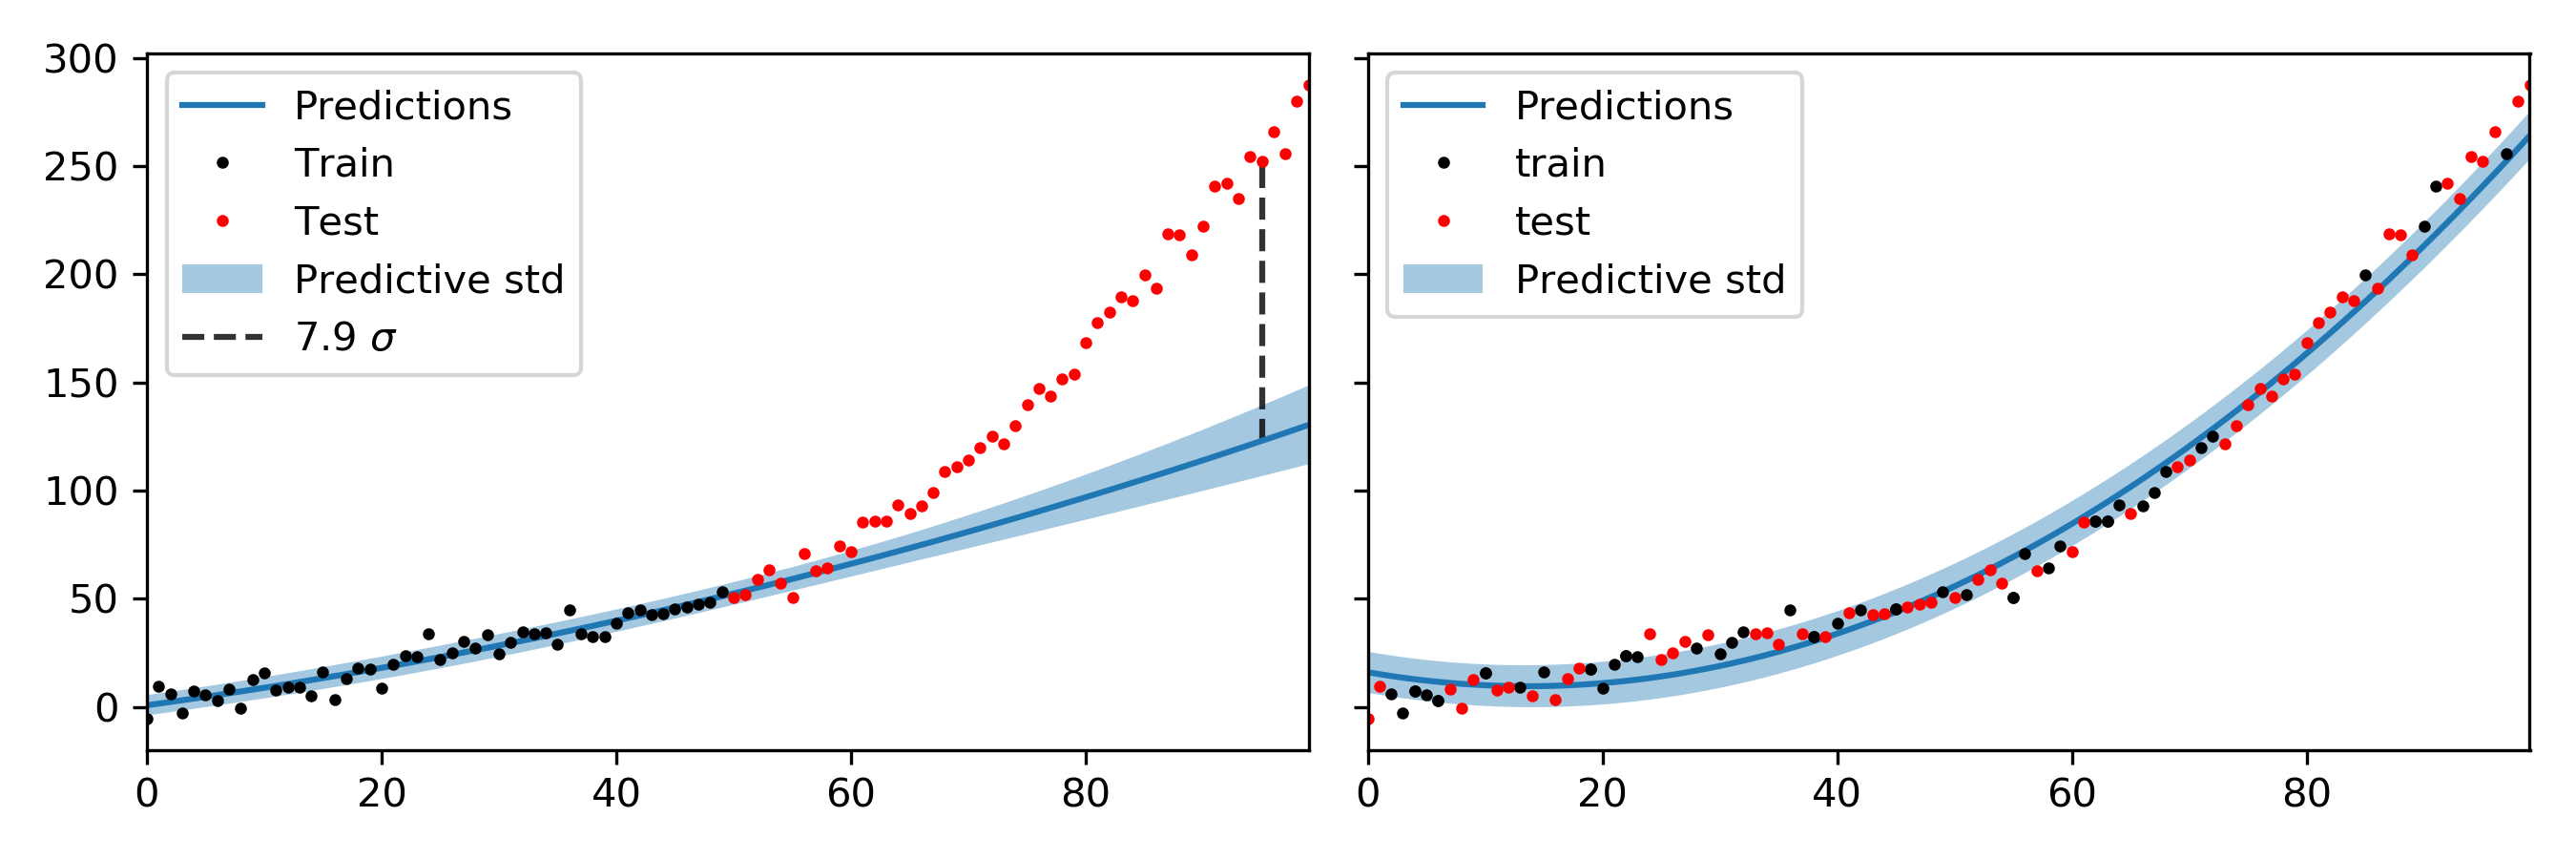
\includegraphics[width=1\textwidth]{Background/BayesianRidge2.png}
    \caption{Quadratic Bayesian regression fitted on different samples from the same dataset}
    \label{fig:bayesian_ridge}
\end{figure}

The models shown in \cref{fig:bayesian_ridge} the models were both trained with fifty samples, which may seem unfair to the model with biased sampling. 
To further highlight the importance of the i.i.d assumption, \cref{fig:bayesian_ridge_low}, shows the two runs of the same model, each trained with only ten i.i.d samples. With only one fifth of the number of samples, we still get decent results, provided they are i.i.d. On the other hand, when the training data does not cover a certain region of input space, we cannot trust the epistemic uncertainty as estimated by \cref{eq:bayesian_predictive}.

\begin{figure}
    \centering
    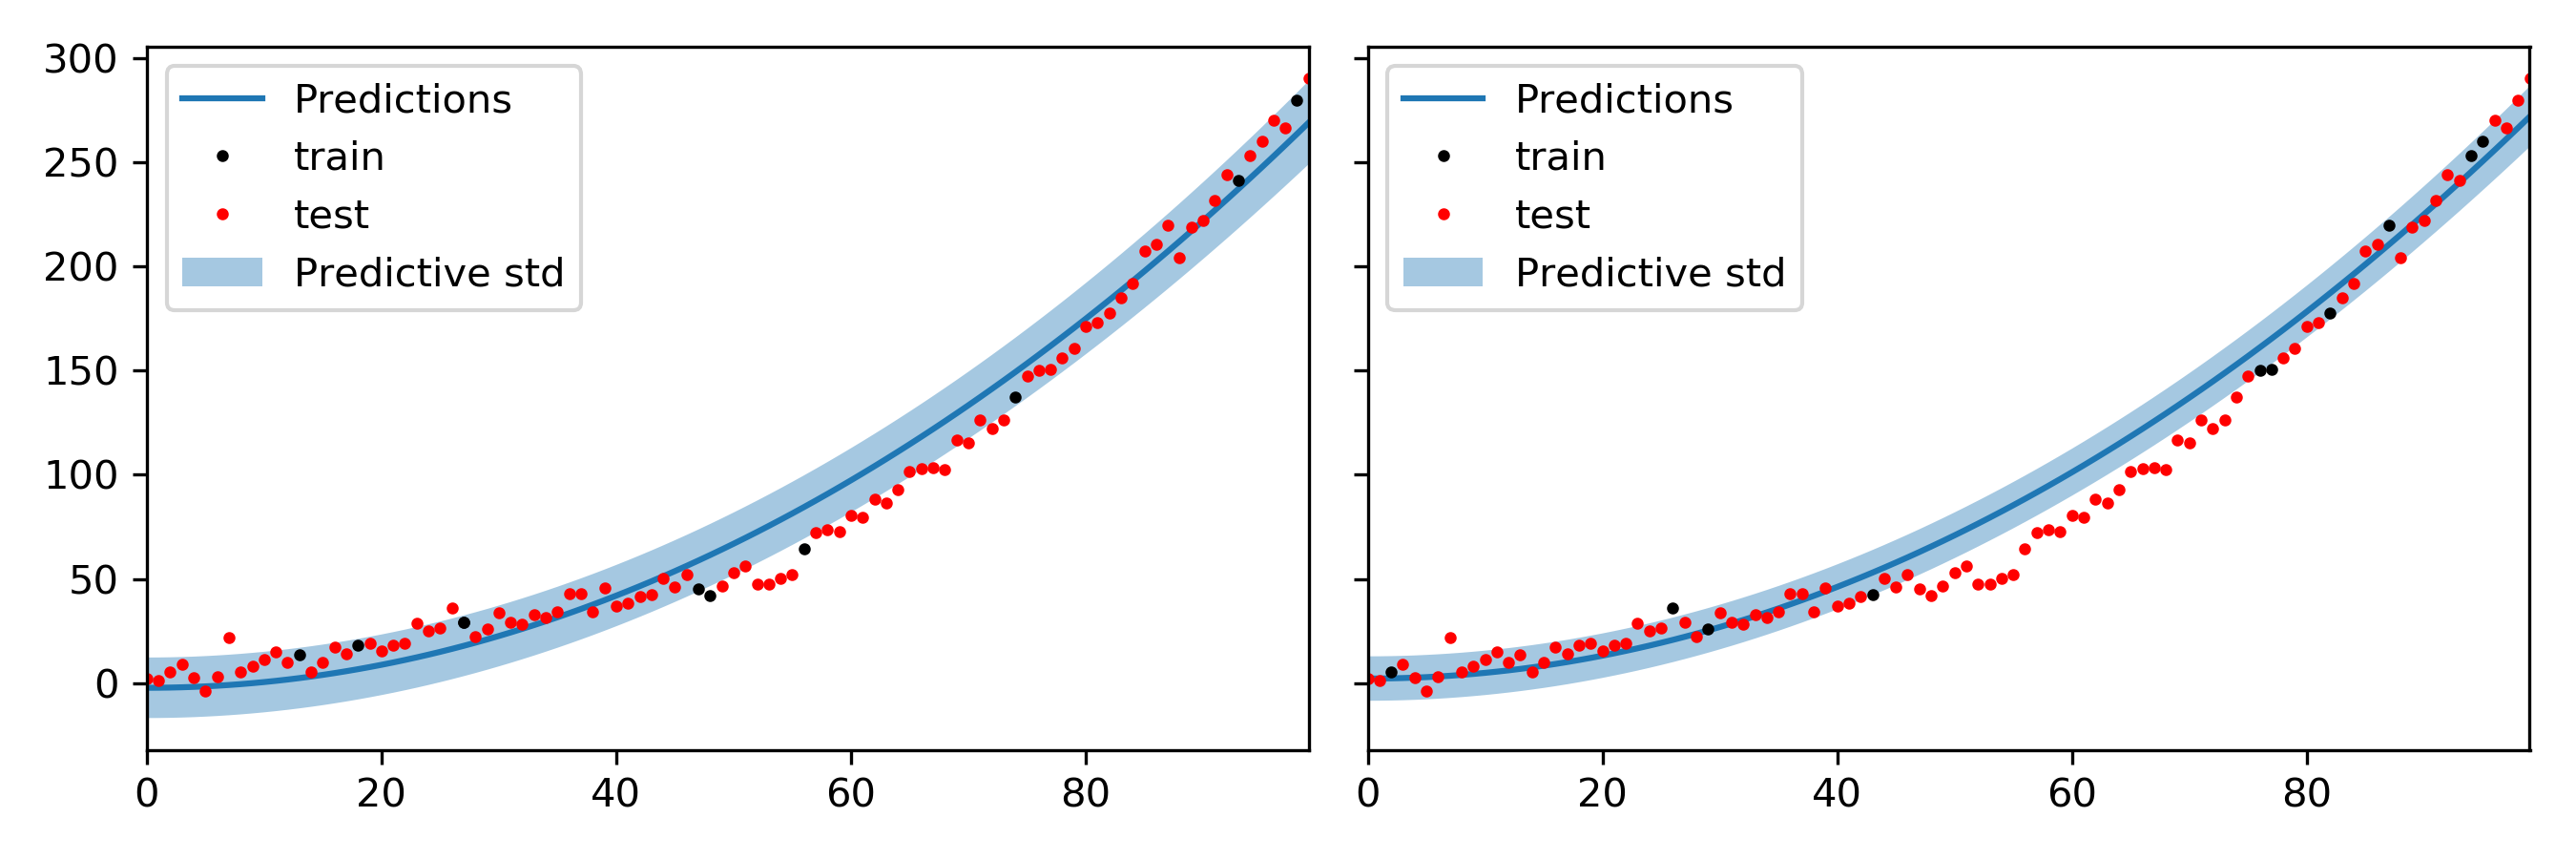
\includegraphics[width=1\textwidth]{Background/BayesianRidgeLow.png}
    \caption{Quadratic Bayesian regression fitted with only 10 i.i.d samples}
    \label{fig:bayesian_ridge_low}
\end{figure}


In our running example of estimating vehicle velocity from sensor measurements. 
Suppose we train a model using data collected on dry roads. the car driving on icy roads is an example of being OOD.
The question again is how valid is our estimate of epistemic uncertainty for OOD inputs. Let us take the case where our hypothesis space contains a model perfect on dry roads, another perfect on icy roads, and all other models have decent performance over both. Assume a uniform prior. Training on dry roads data alone, we eventually end up placing all the posterior mass on the dry roads models.
This drives our epistemic uncertainty, as estimated in \cref{eq:bayesian_predictive}, down to zero everywhere. This means we will be making confident predictions on icy roads, although our predictions for icy road are potentially inaccurate. 

The takeaway is that our uncertainty estimate is not complete for OOD data. The model will be confidently wrong on icy roads. How much we can trust this estimate in practice depends on the hypothesis space, priors, and the behavior of \pdf{y|x}. In the next section, we will formalize the learning setting we discussed here, and discuss a principled approach to handling it.





